% file: atomic-register-case-write-different.tex

\documentclass{standalone}

\usepackage{tikz}
\usepackage{tikz-qtree}

\usetikzlibrary{positioning, shapes, arrows.meta, backgrounds, fit,
	decorations.markings, decorations.pathmorphing}

\begin{document}
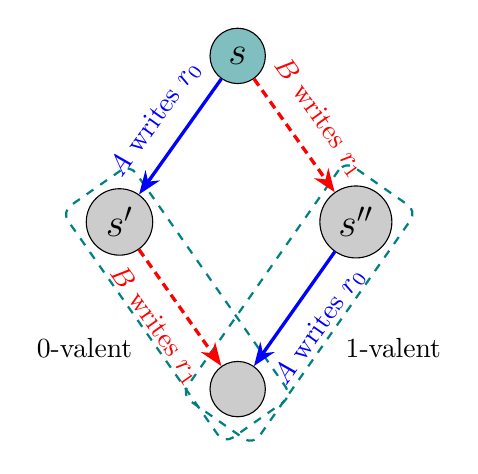
\begin{tikzpicture}[
  univalent/.style = {fill = gray!40},
  bivalent/.style = {fill = teal!50},
  state/.style = {draw, dashed, thick, rectangle, rounded corners, teal, inner sep = 5pt},
  valent/.style = {draw, dashed, very thick, rectangle, rounded corners, green, inner sep = 3pt},
  every tree node/.style = {draw, circle, minimum size = 20pt, font = \Large},
  level distance = 60pt, sibling distance = 60pt,
  edge from parent/.style = {blue, draw, very thick, >=Stealth, ->,
    edge from parent path = {(\tikzparentnode) -- (\tikzchildnode)}}, 
  amove/.style = {},
  bmove/.style = {red, densely dashed},
  cmove/.style = {green, densely dotted},
  chosen/.style = {decorate, decoration = {snake, amplitude = 0.5mm}},
  blank/.style = {draw = none, fill = none},
  txt/.style = {sloped},
]

\Tree [.\node (r) [bivalent] {$s$}; 
  \edge [] node [txt, above = 3pt] {$A$ writes $r_0$};
  [.\node (rl) [univalent] {$s'$};
  ]
  \edge [bmove] node [txt, above = 3pt] {$B$ writes $r_1$};
  [.\node (rr) [univalent] {$s''$};
  ]
]

\node (t) [below = 100pt of r, every tree node, univalent] {};
\draw [edge from parent, bmove] (rl) to node [txt, below = 3pt] {$B$ writes $r_1$} (t);
\draw [edge from parent] (rr) to node [txt, below = 3pt] {$A$ writes $r_0$} (t);

\begin{pgfonlayer}{background}
  \node [rotate fit = 35, fit = (rl) (t), state, label = {180: {$0$-valent}}] {};
\end{pgfonlayer}

\begin{pgfonlayer}{background}
  \node [rotate fit = 55, fit = (rr) (t), state, label = {-90: {$1$-valent}}] {};
\end{pgfonlayer}
\end{tikzpicture}
\end{document}
